\chapter{Literature Review}
The focus of this technical investigation was to develop my knowledge of the NoSQL and indexing solutions examined in the project and to gain insight into the subject matter by reflecting on previously conducted research. Prior to this research, my understanding of the functionality provided by Neo4j and Apache Cassandra was minimal. Throughout my university degree I have undertaken modules which have stipulated a working knowledge of MySQL as a prerequisite therefore my comprehension of MySQL is proficient. - EXPAND
To deliver an all round level of comprehension the following section discusses generic terms which are used throughout the project such as Big Data (Section \ref{bigdata}) and Extract Transform Load (Section \ref{etl}) \textcolor{red}{*FIX*}

\section{Big Data}\label{bigdata}
Big Data is a broad evolving term bound to a complex and powerful application of analytical insight which over recent years has had a variety of definitions. In simplistic terms Big Data can be described as extremely large datasets that may be studied computationally to reveal patterns, trends, and associations for ongoing discovery and analysis.

\subsection{5vs Model}
In 2001, Gartner analyst Doug Laney delivered the original 3vs model which define the challenges and opportunities which have arisen by the increase in data volumes. Laney categorises big data in to three dimensions; Volume, Velocity and Variety, with the increase of each encapsulating the challenges currently faced today of big data management. The characteristics of each property are defined as \textbf{Volume} - Refers to the bast amounts of data generated every second. With the creation and storage of large quantities of data, the scale of this data becomes progressively vast. \textbf{Velocity} - Refers to the speed at which new data is generated and the speed at which data moves around emphasising the "timeliness" of the big data. In order to fully profit from the commercial value of big data, data collection and data examination must be conducted promptly . \textbf{Variety} - This characteristic alludes to the various types of data we can now use; semi-structured and unstructured. Examples being "audio, video, webpage and text as well as traditional structured data" (Chen, Mao, Zhang and CMeung REF).

The amount of data being produced has dramatically increased from when Laney first brought us the 3vs model in 2001. Big Data is a term becoming more and more common in business and society. Overcoming obstacles and implementing effective, actionable Big Data strategies is key for successful big data management. IBM has introduced a fourth V, Veracity \textbf{Veracity} Data inconsistencies and incompleteness result in data uncertainty and unreliability. This creates a new challenge; keeping data organised. (Big Data ref)

The final and considered by many to be the most important V of big data is Value. "All the volumes of fast-moving data of different variety and veracity have to be turned into value" (IBM ref) One of the biggest challenges faced by organisations is having the ability to turn data into value. \textbf{Value} Refers to ones ability to turn big data into something useful and which adds value to your organisation.

\textcolor{red}{\section{Extract Transform Load}}\label{etl}
A basic definition of the Extract Transform Load (ETL) process is pulling data out of one database, refactoring the composition of the data and putting the data into another database. - EXPAND

\subsection{Process}
ETL is a three step procedure which combines database functions into one tool. - EXPAND

\subsubsection{Extract} is the first step in the ETL procedure in which data is read from a database. The Extract step covers the data extraction from the source system and makes it accessible for further processing. The main objective of the extract step is to retrieve all the required data from the source system with as little resources as possible. The extract step should be designed in a way that it does not negatively affect the source system in terms or performance, response time or any kind of locking.

\subsubsection{Transform} where the extracted data is manipulated from its previous state and converted into another database format. The transform step applies a set of rules to transform the data from the source to the target. This includes converting any measured data to the same dimension (i.e. conformed dimension) using the same units so that they can later be joined. The transformation step also requires joining data from several sources, generating aggregates, generating surrogate keys, sorting, deriving new calculated values, and applying advanced validation rules.

\subsubsection{Load} completes the three step procedure and is where data is written into the target database. During the load step, it is necessary to ensure that the load is performed correctly and with as little resources as possible. The target of the Load process is often a database. In order to make the load process efficient, it is helpful to disable any constraints and indexes before the load and enable them back only after the load completes. The referential integrity needs to be maintained by ETL tool to ensure consistency.

\subsection{Tool Implementation}
https://jena.apache.org/
EXPAND

\section{NoSQL}
NoSQL is labeled as a next generation database known to most as "Not only SQL" (NOSQL REF). This definition however insinuates its defiance against the once industry standard SQL. It was originally developed in 1998 by Carlo Strozzi; a member of the Italian Linux society, with the intention of being a non-relational, widely distributable and highly scalable database. Strozzi named the database management system NoSQL to merely state it does not express queries in the traditional SQL format. Sadalage and Fowler believe the definition we commonly refer NoSQL as comes from a 2009 conference in San Fransisco held by Johan Oskarsson, a software developer. Sadalage and Fowler recall Oskarssons desire to generate publicity surrounding the event and in an attempt to do so devised the twitter hashtag "NoSQL Meetup". The main attendees at the conference debrief session were Cassandra, CouchDB, HBase and MongoDB and so the association stuck. (Sadalage and Fowler ref)

There are are number of key features which encompass the NoSQL framework and encapsulate the essence of its popularity. Many of the NoSQL databases boast their capacity of working in a cluster environment - a cluster being two or more connected computers working collaboratively. Thus delivering a range of options for consistency and distribution (Sadalage and Fowler ref) (Section \ref{distributeddb}).

NoSQL solutions are not bound by a definitive schema structure. This permits the ability to freely adapt database records or add custom fields for example without considering structural changes. This is extremely effective when dealing with varying data types and data sets, in comparison to the traditional relational database model which when tackling this issue often resulted in ambiguous field names. (Sadalage and Fowler ref)

\section{Database Classification}
One of the first decisions to be made when when selecting a database is the characteristics of the data you are looking to leverage. (Dash, 2013) There are a multitude of options available with many different classifications. - \textcolor{red}{EXPAND}

\subsection{Distributed Database}\label{distributeddb}
\begin{wrapfigure}{r}{0.5\textwidth}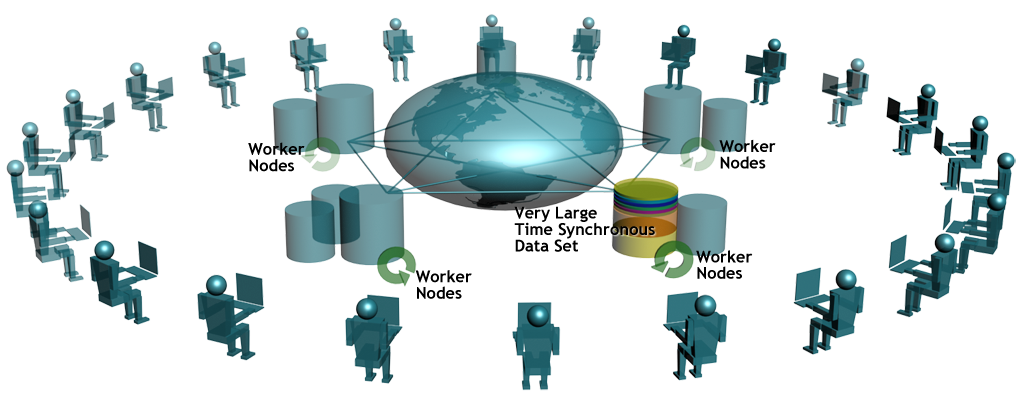
\includegraphics[width=0.9\linewidth]{images/ddelogo}\end{wrapfigure} A distributed database (DDB) comprises of two or more data files located at different sites and servers on a computer network. (DD ref) The advantage of using a DD is that as the database is distributed, multiple users can access a portion of the database at different locations locally and remotely without obstructing one another's work. It is  pivotal for the DD database management system to periodically synchronise the scattered databases to make sure that they all have consistent data. (DD ref) For example if a user updates or deletes data in one location is is essential this change is mirrored on all databases. This ability to remotely access a database from all across the world lends itself to not only multinational companies for example but also startup businesses which recruit the expertise of others from various locations.

\subsection{Document-Oriented Database}
Document-orientated database (DODB) are designed for storing, retrieving and managing document files such as XML, JSON and BSON. The documents stored in a DODB model are data objects which describe the data in the document, as well as the data itself. - EXPAND

\subsection{Graph-Orientated Database}
A graph-oriented database (GODB), is a form of NoSQL database solution that uses graph theory to store, map and query relationships. A graph is a collection of nodes connected by relationships. "Graphs represent entities as nodes and the ways in which those entities relate to the world as relationships." (Robinson, Webber and Eifrem, 2015) The formation of the graph database structure is extremely useful and eloquent as it permits clear modelling of a vast and often ecliptic array of data types. (Robinson, Webber and Eifrem, 2015) An example of data represented in a graph structure is the Twitter relationship model. \begin{center}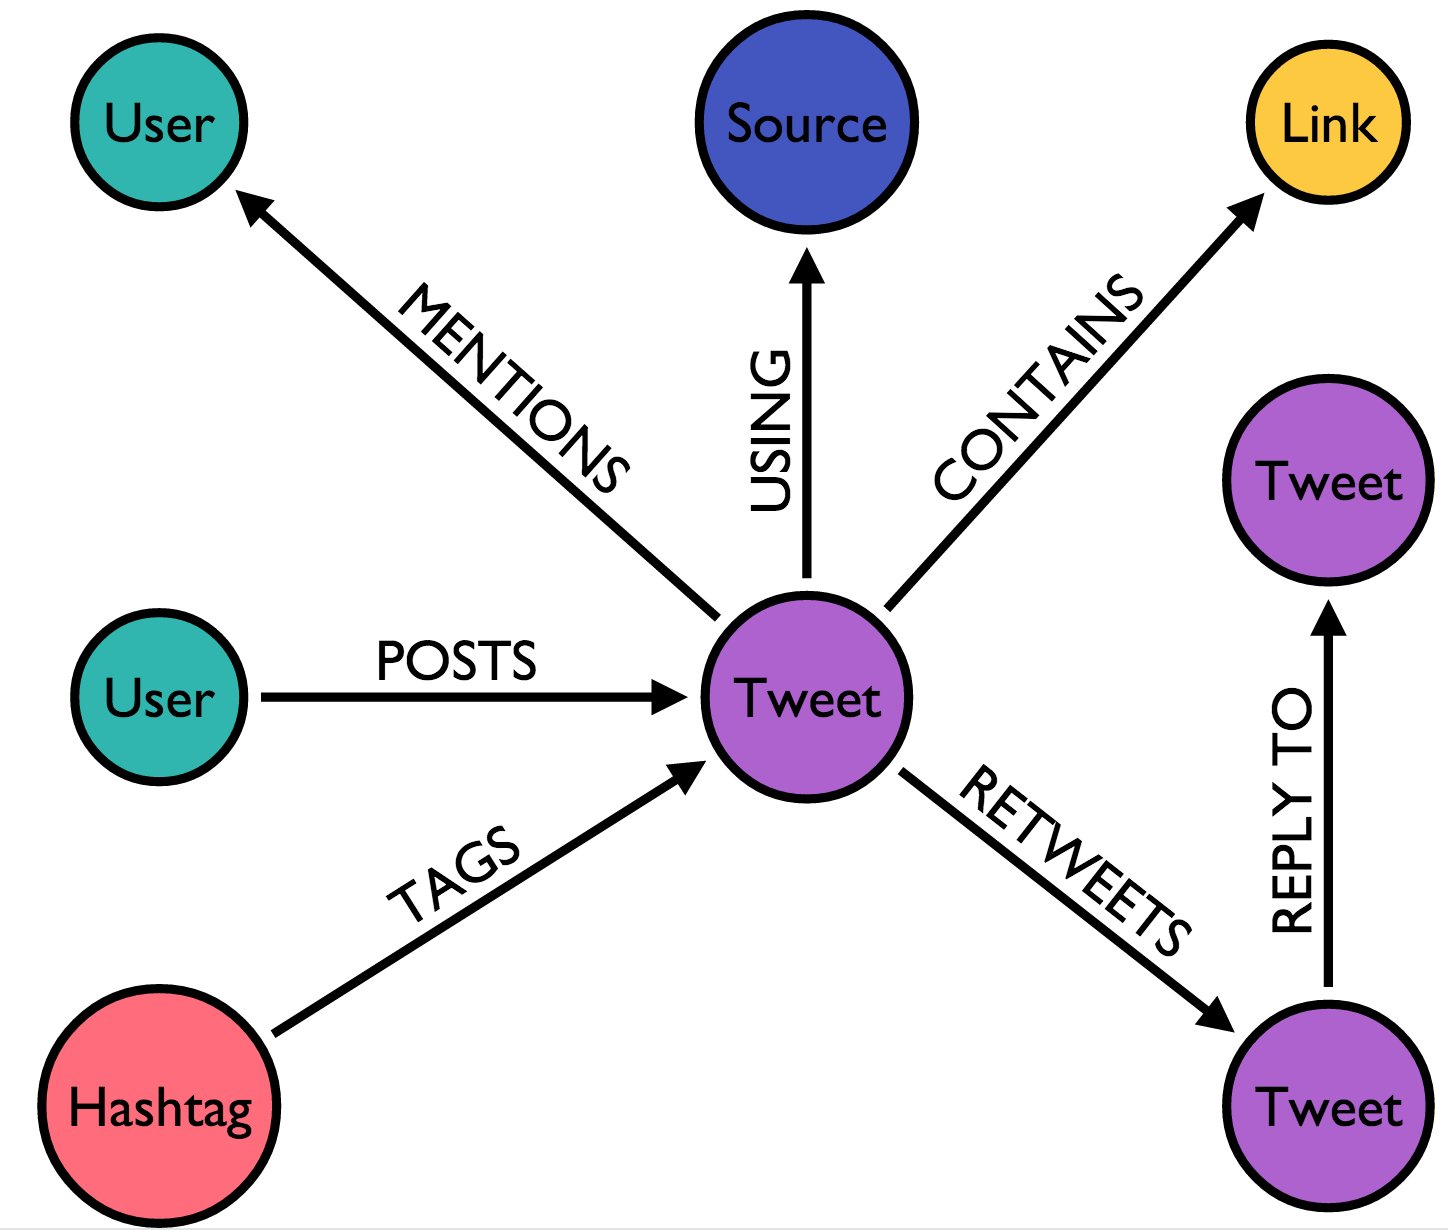
\includegraphics[width=0.3\linewidth]{images/graphdb_twitter}\end{center}  Figure[ADD FIGURE REF] illustrates the nodes involved in a standard tweet and the relationship link between them. The labeled nodes indicate the various operations which are involved in one the tweet. One interpretation of the [FIGURE REF] example is that a user posts a tweet, using the Twitter App which mentions another user and includes a hashtag and link. - \textcolor{red}{REVISE}

\subsection{Relational Database}
A relational database (RDB) is a collection of data items organised as a set of tables, records and columns from which data can be accessed or reassembled in many different ways. (RDB ref) The connected tables are known as relations and contain one or more columns which comprise of data records called rows. Relations can also be instantiated between the data rows to form functional dependencies called keys which are classified as : (RDB ref 2)

\begin{itemize}
\item One to One: One table record relates to another record in another table.
\item One to Many: One table record relates to many records in another table.
\item Many to One: More than one table record relates to another table record.
\item Many to Many: More than one table record relates to more than one record in another table.
\end{itemize}
\section{Proposed Technologies}
The technologies being used in this project are outlined below. \textcolor{red}{EXPAND}
\subsection{MongoDB}\label{mongo}
One of the most popular NoSQL technologies is MongoDB. MongoDB is an open source cross-platform DODB. The premise for using MongoDB is simplicity, speed and scalability (MongoDB White Paper, 2015). Its ever growing popularity, specifically amongst programmers, stems from the unrestrictive and flexible DODB data model which gives you the ability to query on all fields and boasts instinctive mapping of objects in modern programming languages. (MongoDB White Paper, 2015) The database design of MongoDB is based on the JSON file format named BSON.

*NOTES* A record in MongoDB is stored in collections. A collection is a grouping of MongoDB documents.
Within this free flowing environment documents can become as sophisticated and complex as required; information about a document record can be sub categorised by the integration of nested data. *NOTES*

\subsection{Neo4j}\label{neo}
Neo4j is an open-source NoSQL GODB which imposes the Property Graph Model throughout its implementation. The team behind the development of Neo4j describe it as an "An intuitive approach to data problems"(Neo4j web ref). One of the reasons in which Neo4j is favoured predominantly amongst database administrators and developers is its efficiency and high scalability. This is in part due to its compact storage and memory caching for the graphs. "Neo4j scales up and out, supporting tens of billions of nodes and relationships, and hundreds of thousands of ACID transactions per second."(Neo4j web ref) -\textcolor{red}{ FINISH WRITNG UP NOTES}

\subsection{Apache Cassandra}\label{cassandra}
\textcolor{red}{WRITE UP NOTES}

\textcolor{red}{\subsection{MySQL}\label{mysql}}
MySQL is a freely available open source Relational Database Management System (RDBMS) that uses Structured Query Language (SQL).

\section{Data Source and Representation}
The dataset used as a resource to populate the database solutions is called EMAP; a freely available anatomical ontology of the developmental stages of mouse embryos. The EMAP dataset was chosen for this project as my supervisor has much experience in the field and would be able to assist me with any queries I had regarding the data. The size and granularity of the EMAP dataset also meets the criteria which will be required to test the database solutions (Section REQUIREMENTS), explore the limitations of each database comparatively and pose insight into the overall performance of each database.

\subsection{EMAP}
The \textit{Edinburgh Mouse Atlas Project} (EMAP) is an ongoing research project to develop a digital atlas of mouse development. The objective of the EMAP is to implement a digital model of mouse embryos for each time stage in development (EMAP Ref). The collated model embryo data is then used to form a database from which further research can be conducted and experiments can be mapped.
 
Each time step in the digital model are named \textit{Theiler Stages} inspired by the research conducted by Karl Theiler (REF). A Theiler Stage defines the development of a mouse embryo by the form and structure of organisms and their specific structural features. (Theiler Ref) There are 26 individual Theiler Stages which define the growth and evolution of the mouse embryo. The Theiler Stage scheme comprises of both the anatomical developmental stage definition and the estimated length of time since conception. Each Theiler Stage also provides a brief description of the anatomy and any significant changes between the current and previous stage.

Theiler proposed using this scheme as embryos at the same developmental age can have evolved at different rates and therefore exhibit different structural characteristics. (REF Theiler 1989) The EMAP has developed a collection of three dimensional computer models which illustrate and summarise each Theiler Stage. (EMAP website link). 

The anatomy generated at each Theiler Stage has an associated ontological representation. Each provides an alternative aspect of the evolution of a mouse embryo which corresponds with a respective Theiler Stage. The abbreviated term EMAP carries a certain amount of ambiguity as it is refers to the name of the project, and one of the stages in the implemented anatomy. (Ref Ken thesis)  For the purpose of this project the main anatomy to be utilised is the aggregated non stage specific Edinburgh Mouse Atlas Project Abstract (EMAPA) anatomy. The reasoning behind this and comparative ontological anatomies such as EMAP and Edinburgh Mouse Atlas of Gene Expression (EMAGE) are discussed below.

\subsection{EMAP anatomy}
The EMAP anatomy ontology was originally developed to deliver a stage-specific anatomical structure for the developing laboratory mouse. As the EMAP research has progressed, the ontology has followed suit, and is continually under development.

The original EMAP anatomy ontology consists of a series of relational components organised in a hierarchical tree structure which utilise "part-of" relations and subdivisions which encompass each Theiler Stage.(EMAP REF) The intention behind the implementation of the original ontology structure was to "...describe the whole embryo as a tree of anatomical structures successively divided into non-overlapping named parts". (EMAP REF)

Each of the Theiler Stage components has an appropriately named term label, known as the \textit{short name} which describes each respective component. Each Theiler Stage also has a \textit{full name} which comes in the form of the components entire hierarchical path (EMAP REF). Neither the \textit{full} nor \textit{short} anatomical name of each component are required to be distinct and can appear in several Theiler Stages. Therefore to avoid ambiguity each component can be addressed by a unique identifier. The unique identifier is in the form of the relevant anatomy followed by a number (EMAP:number). For example "choroid plexus" is the short name of TS20/mouse/body region/head/brain/choroid plexus and has a has unique identifier of EMAP:4218.

The EMAP hierarchical structure facilitates the need for basic "data annotation and integration" however a combination of the lack of hierarchical views, missing or poorly represented Theiler Stages and label name ambiguity exposed the limitations of the EMAP structure. As a result the need for a hybrid "abstract" version of the anatomy was identified and subsequently developed; EMAPA. (EMAP REF) Thus the EMAPA anatomy will be the main data source for this work.

The research surrounding the EMAP resource is continually being developed, thus the growth of the project as a whole is progressively increasing with the richness of data at the heart (EMAP REF). The EMAPA ontology discussed below (Section \ref{emapaanatomy} is now considered the primary data source thus the EMAP dataset is only available in a combined EMAP and EMAPA standard ontological format developed by the Open Biological Ontologies (OBO) consortium (Section \ref{obo}).


\subsection{EMAPA anatomy}\label{emapaanatomy}
The EMAPA is a refined and algorithmically developed non-stage specific anatomical ontology \textit{abstract} representation of the EMAP anatomy. The EMAPA implementation replaces the EMAP hierarchical tree structure for a \textit{directed acyclic graph} structure; a graph in which it is impossible to start at some vertex v and follow a sequence of edges that eventually loops back to v again.(GRAPH REF) Thus enabling the ability to represent multiple parental relationships and other forms of "is-a" relations where appropriate. (EMAP REF)

Each anatomical component in the EMAPA anatomy is identified as a single term, coupled with the appropriate start and end Theiler Stage at which the component is considered to be present in the developing embryo. (EMAP REF) With the aim of enhancing user experience, the EMAPA anatomy  implements an alternative naming convention from the EMAP anatomy replacing full path names for components to \textit{"print names"}. Using the above example for comparison, "EMAP:4218" in the EMAP anatomy becomes "TS20 brain choroid plexus" in EMAPA. This naming convention supplements the requirement of uniqueness and is easily comprehensible.

The EMAPA ontology is available in a standard ontological format developed by the Open Biological Ontologies (OBO) consortium (Section \ref{obo}) and is also available in a Web Ontology Language (OWL); a standard produced from W3C (Section \ref{owl}).This enhanced OWL version of the ontology is now considered as the primary EMAP anatomy ontology and thus will be the main source for the work on this project. 


\subsection{EMAGE anatomy}
\subsection{Data Representation Languages}
\subsubsection{EMA Database}\label{emadb}
\subsubsection{Web Ontology Language OWL}\label{owl}
%http://www.w3.org/TR/2004/REC-owl-guide-20040210/#Introduction
The Web Ontology Language OWL is language representation standard for designing and instantiating ontologies produced from the World Wide Web Consortium W3C. The OWL file format is designed to be humanly readable and also recognisable to applications required to process the content of the information. "[OWL] is intended to provide a language that can be used to describe the classes and relations between them that are inherent in Web documents and applications." (OWL REF). 
\subsubsection{OBO}\label{obo}
The OBO flat file format is an ontology representation language (OBO ref)

